% Conceptual sensitivity analysis, annotated version
% USe pts from dev/conceptual-sensitivity-analysis-curves.R.
% Palettes: c("#2f6f9f", "#c1531f", "#3f8f5b", "#8a5cb0", "#b0842f")
\documentclass[tikz,border=6pt]{standalone}
\usepackage{pgfplots}
\pgfplotsset{compat=1.18}
\usetikzlibrary{arrows.meta}
\definecolor{steelblue}{RGB}{70,130,180}
% Scenario colors match viridis::viridis(4) in
% conceptual-sensitivity-analysis-curves.R
\definecolor{scenBase}{HTML}{2f6f9f}      % Base scenario
\definecolor{scenSlower}{HTML}{c1531f}    % Slower
\definecolor{scenFixedGamma}{HTML}{3f8f5b}% Fixed gamma (beta=1.74, off axis)
\definecolor{scenFixedBeta}{HTML}{8a5cb0} % Fixed beta

\begin{document}
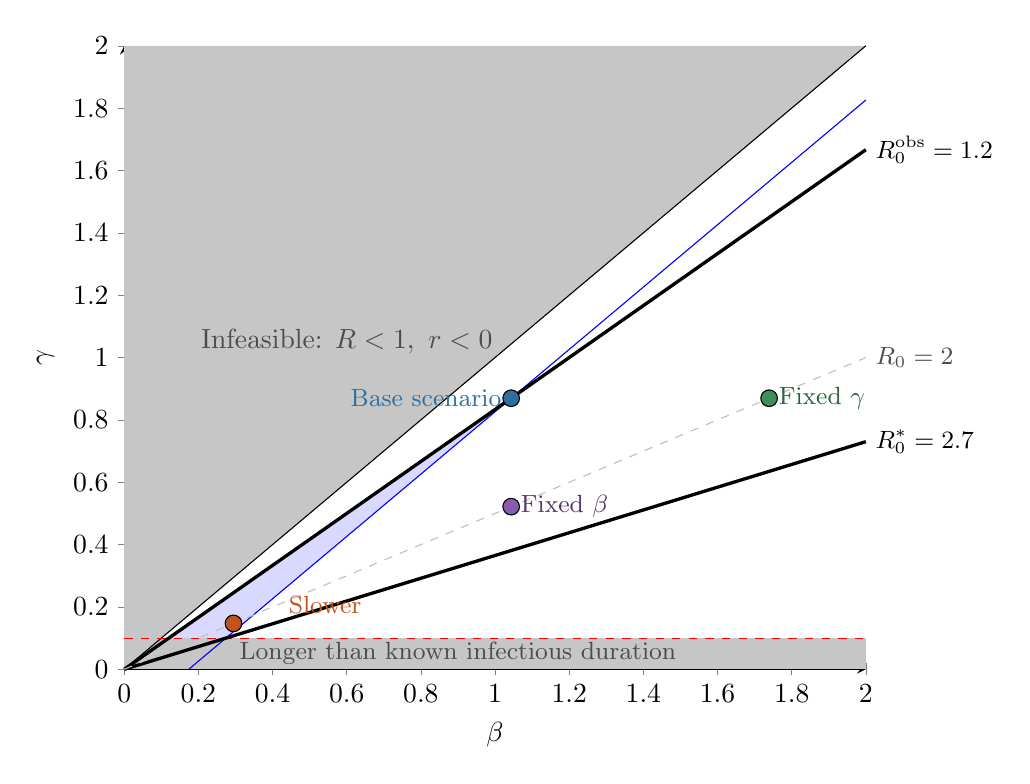
\begin{tikzpicture}
  \begin{axis}[
      width=11cm, height=9.5cm,
      xmin=0, xmax=2, ymin=0, ymax=2,
      xlabel={$\beta$}, ylabel={$\gamma$},
      axis lines=left,
      clip=false,
      enlargelimits=false,
    ]

    % Grayed-out region above the y = x line (R < 1, r < 0)
    \addplot[gray!45, fill=gray!45, draw=none]
      coordinates {(0,0) (2,2) (0,2)} -- cycle;

    % Grayed-out infeasible region below gamma_max
    \addplot[gray!45, fill=gray!45, draw=none]
      coordinates {(0,0) (2,0) (2,0.1) (0,0.1)} -- cycle;

    % Shaded "slower" triangle
    \addplot[steelblue, fill=blue!15, draw=none]
      coordinates {(0.12,0.1) (0.273913,0.1) (1.043478,0.869565)} -- cycle;

    % Reference lines
    \addplot[black, thin] coordinates {(0,0) (2,2)};               % y = x
    \addplot[red, dashed] coordinates {(0,0.1) (2,0.1)};           % gamma_max
    \addplot[blue] coordinates {(0.173913,0) (2,1.826087)};        % r = r.hat
    \addplot[black, very thick]
      coordinates {(0,0) (2,0.730159)};                            % R0.predict
    \addplot[black, very thick]
      coordinates {(0,0) (2,1.666667)};                            % R0.hat
    \addplot[gray!50, dashed] coordinates {(0,0) (2,1)};           % R0 = 2

    % Scenario points (locations from conceptual-sensitivity-analysis-curves.R).
    \addplot[only marks, mark=*, mark size=3pt, scenBase, draw=black]
      coordinates {(1.043478,0.869565)};                 % Base scenario
    \addplot[only marks, mark=*, mark size=3pt, scenSlower, draw=black]
      coordinates {(0.29459,0.147295)};                 % Slower
    \addplot[only marks, mark=*, mark size=3pt, scenFixedGamma, draw=black]
      coordinates {(1.739130,0.869565)};                 % Fixed gamma
    \addplot[only marks, mark=*, mark size=3pt, scenFixedBeta, draw=black]
      coordinates {(1.043478,0.521739)};                 % Fixed beta
    

    % Scenario labels
    \node[anchor=east, font=\small, scenBase] at (axis cs:1.043478,0.869565)
      {Base scenario};
    \node[anchor=north west, font=\small, scenSlower]
      at (axis cs:0.417619,0.265945) {Slower};
    \node[anchor=west, font=\small, scenFixedGamma!70!black]
      at (axis cs:1.739130,0.869565) {Fixed $\gamma$};
    \node[anchor=west, font=\small, scenFixedBeta!60!black]
      at (axis cs:1.043478,0.521739) {Fixed $\beta$};

    % Region labels
    \node[gray!60!black] at (axis cs:0.6,1.05) {Infeasible: $R < 1,\ r < 0$};
    \node[gray!60!black, font=\small, align=center]
      at (axis cs:0.9,0.05)
      {Longer than known infectious duration};
    %\node[font=\bfseries] at (axis cs:0.479,0.357) {slower};

    % Line-end labels (R0 = 1.2 corresponds to R0.hat)
    \node[anchor=west, font=\small] at (axis cs:2,1.666667)
      {$R_0^\mathrm{obs} = 1.2$};
    \node[anchor=west, font=\small] at (axis cs:2,0.730159)
      {$R_0^\ast = 2.7$};
    \node[anchor=west, font=\small, gray!60!black] at (axis cs:2,1)
      {$R_0 = 2$};

  \end{axis}
\end{tikzpicture}
\end{document}
